\documentclass[12pt, a4paper]{article}

\usepackage[czech]{babel}
\usepackage[T1]{fontenc}
\usepackage[utf8]{inputenc}
\usepackage{enumitem}
\usepackage{parskip}
\usepackage{tocloft}
\usepackage{multicol}
\usepackage[hidelinks]{hyperref}
\usepackage{graphicx}
\usepackage{float}
\usepackage{listings}
\usepackage{xcolor}
\usepackage{listings}
\usepackage{fontawesome}

\begin{document}

\begin{titlepage}
    \begin{center}
        
        
        \vspace{2cm}
        
        \Huge
        \textbf{UPS - Semestrální práce}
        
        \vspace{1cm}
        
        \LARGE
        Protokol pro hru kostky (Dice/Farkle)
        
        \vfill
        
        \vspace{0.5cm}
        
        \normalsize
        \raggedright
        Vypracoval: Martin Schön \\
        Studijní číslo: A22B0144P \\
        Datum: \today
        \vspace{0.2cm}
        
    \end{center}
\end{titlepage}
\thispagestyle{empty}
\pagebreak

%tečky v obsahu
\renewcommand{\cftsecleader}{\cftdotfill{\cftdotsep}}
\renewcommand{\cftsubsecleader}{\cftdotfill{\cftdotsep}}
\renewcommand{\cftsubsubsecleader}{\cftdotfill{\cftdotsep}}

%obsah
\setcounter{page}{2}
\tableofcontents
\pagebreak


\section{Úvod}
Tento dokument popisuje protokol TCP pro hru kostky (Dice/Farkle). 
Protokol není zcela kompletní, nejsou zde popsány všechny možné stavy a chyby, které mohou nastat.
Protokol je navržen tak, aby byl co nejjednodušší a zároveň dostatečně robustní pro hru kostky.


\section{Struktura zprávy}
Zpráva je posílána v textové podobě. 
Zpráva je rozdělena na několik částí, které jsou odděleny znakem \texttt{':'} a \texttt{';'}.
Znak \texttt{':'} je použit pro oddělení jednotlivých částí zprávy a určení o jakou zprávu se jedná.
Dále odděluje jednotlivé parametry zprávy.
Znak \texttt{';'} je použit pro oddělení jednotlivých částí zprávy, které mohou obsahovat více hodnot.

\section{Zprávy}
Všechny zprávy začínají identifikátorem \texttt{dc:}.
\subsection{Přihlášení hráče}
Ze stavu Login se může hráč dostat do stavu Lobby Table.
\begin{itemize}
    \item \texttt{dc:login:<username>}
    \begin{itemize}
        \item \texttt{username} -- jméno hráče
    \end{itemize}
\end{itemize}

Pokud se hráč odpojí z Lobby Table, vrátí se do stavu Login.
\begin{itemize}
    \item \texttt{dc:logout:<username>}
    \begin {itemize}
        \item \texttt{username} -- jméno hráče
    \end{itemize}
\end{itemize}

\subsection{Lobby}
V lobby Table si hráč vybírá stůl, ke kterému se chce připojit. 
Zároveň může vytvořit nový stůl, který bude mít jeho jméno jako majitele.
Pokud hráč nese stejné jméno jako majitel stolu, může stůl smazat.
Každý vytvořený stůl bude mít uložený dvě jména a to hráčů, kteří se do něj připojí.
\begin{itemize}
    \item \texttt{dc:lobby:create:<table\_name>}
    \begin{itemize}
        \item \texttt{table\_name} -- jméno stolu
    \end{itemize}
    \item \texttt{dc:lobby:delete:<name>}
    \begin{itemize}
        \item \texttt{table\_name} -- jméno stolu
        \end{itemize}
    \item \texttt{dc:lobby:join:<table\_name><username>}
    \item \texttt{dc:lobby:leave:<table\_name><username>}
    \begin{itemize}
        \item \texttt{table\_name} -- jméno stolu
        \item \texttt{username} -- jméno hráče
    \end{itemize}
\end{itemize}

Poslední zpráva je Lobby Fetch, která pošle všechny stoly, které jsou vytvořené.
\begin{itemize}
    \item \texttt{dc:lobby:fetch}
\end{itemize}

\subsection{Game}
V této části jsou zprávy, které se týkají hry.
Tyto zprávy nejsou zcela kompletní, nejsou zde popsány všechny možné stavy a chyby, které mohou nastat.
\begin{itemize}
    \item \texttt{dc:game:throw:<table\_name><username>}
    \begin{itemize}
        \item \texttt{table\_name} -- jméno stolu
        \item \texttt{username} -- jméno hráče
    \end{itemize}
\end{itemize}

Dále zde budou zprávy, které budou obsahovat zkontrolování hodů a zároveň zprávy, které budou obsahovat výsledky hodů.

\subsection{Odpojení}
Pokud se hráč odpojí, bude odstraněn ze stolu a vrátí se do stavu Login.
U hráče, se kontroluje, zda je v Lobby Table nebo ve hře.
Každých 30 sekund se kontroluje, zda je hráč stále připojen.
Pokud hráč není připojen, tak zůstane ve stavu, ve kterém byl, ale po opětovném připojení bude přesunut do stavu Login.
\begin{itemize}
    \item \texttt{dc:disconnect:<username>}
    \begin{itemize}
        \item item \texttt{username} -- jméno hráče
    \end{itemize}
\end{itemize}

\pagebreak
\section{Diagram protokolu}
\begin{figure}[H]
    \centering
    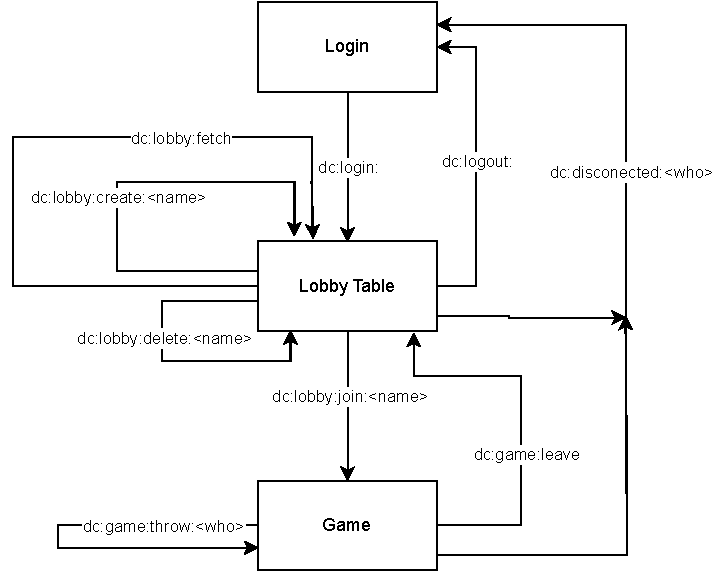
\includegraphics[width=\textwidth]{../protocol_diagram.drawio.pdf}
\end{figure}

\end{document}